\chapter{Implementierung}
\label{implementierung}

In diesem Kapitel wird die Implementierung beschrieben. Zunächst werden die Komponenten und Klassen der Anwendung vorgestellt. Die gezeichneten Mockups unterscheiden sich nur minimal von der tatsächlichen Anwendung. Im Großen und Ganzen ist das Design aber gleich geblieben.

\section{Komponenten}
Die Komponenten bilden alle Funktionen der App, welche visuell auf der Benutzeroberfläche wahrgenommen werden. Neben der Anzeige der Elemente beinhalten sie aber dennoch auch Funktionalität, wie beispielsweise das Aufrufen von Methoden der Datenbank-Klasse ,DbConnectionService'. Alle Komponenten, mit Ausnahme der ,App', besitzen ein eigenes Interface. Dieses Interface beinhaltet alle Elemente, die als Properties in die Komponente hineingegeben werden und die jeweils dazugehörigen Typen. Properties können als Parameter an eine Komponente verstanden werden. Dies können neben Strings, Zahlenwerten oder boolschen Werten auch Funktionen oder andere Objekte sein.
\subsection{Komponente ,App'}
Die ,App'-Komponente kann sozusagen mit der ,main()'-Funktion anderer Programmiersprachen verglichen werden. Alles, was in dieser Funktion seinen Platz findet, findet sich auch in der Anwendung selbst wieder. Alle notwendigen Komponenten, die die Anwendung benötigt, werden hier eingefügt. 

Zu Beginn werden hier die Tabellen der Datenbank erstellt, sofern diese noch nicht existieren. Diese Komponente verwaltet die Daten. Die Informationen zu den Parkmöglichkeiten, die über die API abgerufen werden, werden zudem auch hier verwaltet. Durch den Hook ,useEffect' wird sichergestellt, dass die Daten nach einer bestimmten Zeit erneut abgefragt werden. Der Code hierfür kommt aus dem Internet und ist in \autoref{lst:useEffectApiData} zu sehen.

\begin{lstlisting}[caption={In diesem Hook werden nach der Zeit, welche sich hinter der Variable ,MINUTES\_MS' verbirgt, die Daten der API abgerufen, was über die Funktion in Zeile 3 geschieht. (Quelle: \cite{useIntervalCode})},captionpos=b, language=Java, label=lst:useEffectApiData]
	useEffect(() => {
		const intervalCall = setInterval(() => {
			dbConnectionService.getData();
		}, MINUTES_MS);
		return () => {
			clearInterval(intervalCall);
		};
	}, []);
\end{lstlisting}

Desweiteren gehehn auch die Daten des Eventhooks ,useGeofenceEvent', welcher in \autoref{geofenceEvent} erklärt wird, hier ein. Durch die Properties der anderen Komponenten werden die Daten dann an die richtigen Stellen gebracht. Wird ein Geofence betreten, so geschieht auch hier die Sprachausgabe. Der Button für das Ein- und Ausschalten des Tons befindet sich ebenfalls in der ,App'. Auch die Verwaltung des Tons liegt hier. Wird eine andere Ansicht geöffnet oder der Button zum Stummschalten der Sprachausgabe betätigt, so wird ein ,useEffect'-Hook getriggert, welcher die Sprachausgabe direkt beendet.

Neben verschiedenen ,set'- und ,get'-Funktionen, die für die Weitergabe von Daten zwischen Komponenten verantwortlich sind, befindet sich hier auch das Element, welches benötigt wird, um Toasts auszugeben. Alle Bestandteile in der ,<View>'-Komponente werden von ,<RootSiblingParent>' umrahmt, damit nachher an verschiedenen Stellen der Befehl aus \autoref{lst:toast} aufgerufen werden kann und somit in der Anwendung einen Toast anzeigt \cite{toastLibrary}.

\begin{lstlisting}[caption={Ein Beispiel des Aufrufs eines Toasts aus der Datei DbConnectionService. (Quelle: Eigene Implementierung)},captionpos=b, language=Java, label=lst:toast]
	Toast.show(errorMessages.noApiConnectionMessage, {
		duration: Toast.durations.LONG,
		position: Toast.positions.BOTTOM,
	});
\end{lstlisting}

\subsection{Komponente ,ParkingMap'}
Die wohl wichtigste Komponente der Anwendung ist die, welche die Karte beinhaltet. Diese findet sich hier. Zunächst wird beschrieben, welche Properties mitgeliedert werden. Hierzu ist es hilfreich, das zugehörige Interface ,IParkingMap' mit den Typen der Properties zu betrachten:
\begin{description}
	\item \textbf{handleParkingAreaId(id: number): void} \\ Hineingegeben wird eine Funktion ,handleParkingAreaId', welche nichts zurückgibt. Parameter ist hier ,id', was den Typ Nummer hat. Diese Funktion bringt die jeweilige ID der Parkmöglichkeit nach draußen in die ,App' und kann dort weiterverarbeitet werden.
	\item \textbf{handleParkingAreaDescription(parkingAreaDescription: boolean): void} \\ ,handleParkingAreaDescription' ist eine Funktion, welche nichts zurückgibt. Der Parameter dieser Funktion ist ein boolscher Wert namens ,parkingAreaDescription'. Diese Property hat in etwa denselben Nutzen, wie die eben beschriebene. Nur wird hier der ,App' mitgeteilt, ob die Beschreibung einer Parkmöglichkeit geöffnet werden soll oder nicht.
	\item \textbf{mapStyle: StyleProp<ViewStyle>} \\ Diese Property ist für das Design der ,ParkingMap' verantwortlich. Je nachdem, ob die Beschreibung der Parkmöglichkeit angezeigt wird oder nicht, ist die ,ParkingMap' größer oder kleiner.
\end{description}

Diese Komponete übernimmt die Anzeige der aktuellen Position des Nutzers und das Bilden der Geofences. Damit das funktioniert, benötigt man die Bibliothek Location von expo \cite{expoLocation}. Zur Nutzung von Geofences und der Anzeige der aktuellen Position wird die Erlaubnis des Nutzers für das GPS benötigt. Ohne diese Zustimmung wird dem Nutzer eine Meldung angezeigt, dass weder das Geofencing, noch die Anzeige der aktuellen Position funktionieren.

Um nun auch die Karte und die Marker an den Positionen der Parkhäuser anzeigen zu lassen, werden zusätzlich die Komponenten ,MapView' und ,Marker' der Bibliothek ,react-native-maps' benötigt. Je nach Gerät wird dann bei Android Google Maps und bei IOS Apple Maps verwendet. Um nun die Marker an den richtigen Stellen zu plazieren, wird die Liste aller Objekte der Parkmöglichkeiten mit der Funktion ,map()' durchgegangen und an jeder Stelle der Parkhäuser ein Marker gesetzt. Die Daten der Parkhäuser sind hier nicht aus der Datenbank, sondern aus dem Objekt-Array ,AllParkingAreas', welches in \autoref{AllParkingAreas} näher erklärt wird. Wird auf einen Marker geklickt, kommen die beiden Funktionen der Properties ins Spiel. Der Aufruf der Funktion ,handleParkingAreaId' mit der ID der angeklickten Parkmöglichkeit als Parameter lässt die ,App' wissen, welche Parkmöglichkeit angeklickt wurde. Wenn die Funktion ,handleParkingAreaDescription' mit dem Parameter ,true' aufgerufen wird, wird sichergestellt, dass sich dann immer die Beschreibung, welche in \autoref{fig:parkingAreaDescription} zu sehen ist, öffnet.

\begin{figure}[h!]
	\centering
	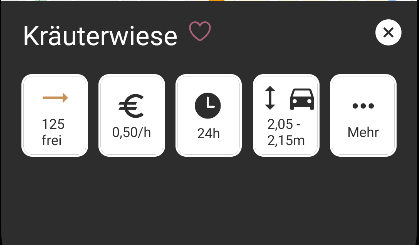
\includegraphics[width=0.45\linewidth]{parkingAreaDescription_component.png}
	\caption[Die Komponente ,ParkingAreaDescription', welche bei Klick auf einen Marker aufgerufen wird.]
	{Die Komponente ,ParkingAreaDescription', welche bei Klick auf einen Marker aufgerufen wird. (Quelle: Screenshot der erstellten Anwendung.)}
	\label{fig:parkingAreaDescription}
\end{figure}

\subsection{Komponente ,ParkingAreaDescription'}
\subsubsection{Komponente ,ParkingAreaDescriptionItemContainer'}
\subsection{Komponente ,ParkingAreaList'}
\subsubsection{Komponente ,ParkingAreaListItem'}
\subsection{Komponente ,ParkingAreaDetails'}
\subsubsection{Komponente ,ParkingAreaDetailsItem'}
\subsection{Komponente ,ParkingAreaListHeading'}
\section{Datenbankverbindung ,DbConnectionService'}
\section{Eventhook ,useGeofenceEvent'}
\label{geofenceEvent}
\section{Models}
\subsection{Interface ,IParkingArea'}
\subsection{Interface ,IParkingAreaDetails'}
\subsection{Interface ,IEventData'}
\section{Parkhausdaten ,AllParkingAreas'}
\label{AllParkingAreas}
\section{Weitere Hilfsmittel}
\subsection{Zentrale Verwaltung der Farben}
\subsection{Zentrale Verwaltung der Strings}